\documentclass[prc,preprint,superscriptaddress,showpacs,floatfix]{revtex4-1}
\usepackage{graphicx,amsmath,amssymb,bm}
\usepackage{braket}
\usepackage{amsfonts}
\usepackage{ucs}
\usepackage{pgf,pgfarrows,pgfnodes,pgfautomata,pgfheaps,pgfshade}
\usepackage{amsmath,amssymb}
\usepackage[latin1]{inputenc}
\usepackage{colortbl}
\usepackage[english]{babel}


\begin{document}

\title{Spectroscopic Information near $N=14$ and $N=16$}

\author{Joe Belarge, Alexandra Gate {\em et al}}
\affiliation{National Superconducting Cyclotron Laboratory, Michigan
  State University, East Lansing, MI 48824-1321, USA}
\affiliation{Department of Physics and Astronomy, Michigan State University, East Lansing, MI 48824, USA}

\maketitle


\section{Physics Motivation}
Historically, the concept of independent particle motion, and various
mean-field approaches based thereupon, has played and continues to
play a fundamental role in studies of quantum mechanical many-particle
systems.  From a theoretical standpoint, a single-particle (or
quasiparticle) picture of states near the Fermi surface offers a good
starting point for studies of systems with many interacting particles.
The success of the nuclear shell model rests on the assumption that
the wave functions used in nuclear structure studies, can be
approximated by Slater determinants built on various single-particle
states.  
In a field like nuclear physics, where the interaction between nucleons is strong, one
expects that correlations beyond the independent particle motion
should play an important role in spectroscopic observables.  
Furthermore, correlations which arise as one moves
towards either the proton or the neutron driplines, can alter strongly 
the interpretation and meaningfulness of a mean field and how shells evolve
towards the limits of nuclear stability. 

Unfortunately, the consequences of correlations in many-particle
systems are normally extremely difficult to measure experimentally and
to interpret theoretically. There are rather few observables from
which one can extract clear information on correlations beyond an
independent particle motion in a nuclear many-body environment.

A quantity which offers the possibility to study deviations from a
single-particle picture, and thereby provide information on
correlations, is the spectroscopic factor (SF). Although not being an
experimental observable {\em per se} the SFs are defined as the ratio
of the observed reaction rate with respect to the same rate calculated
assuming a full occupation of the relevant single-particle
states. They are thus often interpreted as a measure of the occupancy
of a given single-particle state. From a theoretical point of view
they represent a measure of what fraction of the full wave function
can be interpreted as an independent single-particle or hole state on
top of a correlated state, normally chosen to be a closed-shell
nucleus.

Recent advances in {\em ab initio} calculations have resulted in the
ability to calculate the properties of nuclei with mass greater than
20, providing precise estimations of properties of nuclei like
${48}$Ca \cite{naturephysics2015}, employing properly constrained two-
and three-nucleons interactions from effective field theory (and
thereby obeying important symmetries of QCD) \cite{ekstrom2015}. These
advances allow us now to compute nuclear observables of both stable
nuclei and nuclei close to or beyond the driplines, without parameter
fitting \cite{physicascripta2016}. 
Furthermore, recent developments of many-body theory allows us also to compute
more reliably effective Hamiltonians which can be used in a nuclear structure
context \cite{bogner2014,jansen2014,jansen2015}. 
Experimental results on nuclei
close to the driplines provide thus unique inputs to our basic
understanding of correlations in nuclear systems near the limits of
stability.

Experimentally there has been quite some emphasis on neutron-rich
oxygen isotopes recently.  The nucleus $^{24}$O is well established as
the last bound oxygen isotope. Several recent experiments have
provided information on neutron properties close to or beyond the
dripline of oxygen isotopes.

However, there is little known about nuclei one to two protons away
from the potentially doubly magic $^{22}$O and the doubly magic
$^{24}$O.  In the case of $^{22}$O, much has been studied
experimentally with respect to neutron degrees of freedom, with the
primary aim being identifying whether or not the $N=14$ subshell gap
is magic [THI00,STA04,BEC06]. The experimental data, however, is
lacking for nuclei that vary by one proton from $^{22}$O. For example,
since $^{21}$N was first observed in 1970 [ART70] only two experiments
have been performed to identify excited states of this nucleus
[SOH08,ELE10]. In the case of Ref. [SOH08] five excited states were
observed by two step fragmentation and were given tentative
spin-parity assignments. Similarly, excited states have been measured
in $^{23}$F three times [ORR89,AZA02,MIC06]. Most recently a series of
four reactions were used to populate excited states, including single
and multi-nucleon knockout, proton transfer, and inelastic scattering
[MIC06]. These measurements resulted in an analysis of the angular
distributions of charged particles from the ($^{4}$He,$t$) transfer
reaction which led to the determination of spectroscopic factors for
two of the observed states. For both $^{23}$F and $^{21}$N, there are
no firm spin-parity assignments, and spectroscopic factors are either
unknown ($^{21}$N) or unconfirmed ($^{23}$F).  A more thorough study
of the excited states in $^{23}$F and $^{21}$N, including firm
spin-parity assignments and measurements of spectroscopic factors,
would provide invaluable input to our understanding of how a
single-particle interpretation evolves towards the
driplines. Experimental cross sections combined with theoretical {\em ab initio} 
calculations of spectroscopic factors can thus shed
important information on the evolution of shells and proton and
neutron single-particle states close to $^{24}$O.  Approaching the
neutron dripline with $^{24}$O, the experimental data becomes more
scarce. Although $^{25}$F was also first observed in 1970 [ART70] and
several gamma rays were observed in the early 2000s [BEL01,AZA02,ELE04], 
the first detailed spectroscopy of excited states
in $^{25}$F was not published until 2014 [VAJ14]. In Ref [VAJ14] seven
gamma-rays are identified corresponding to five excited states.  The
states are given tentative spin-parity assignments, but due to the
nature of the fragmentation reaction employed, spectroscopic factors
were not determined.  Performing single proton knockout reactions with
beams of radioactive $^{24,26}$Ne and $^{23}$O will provide a critical
means to further develop the current understanding of the structure of
neutron rich isotopes near $N=14$ and $N=16$. By probing the largely
mysterious proton shell structure in this region in a systematic way,
as a function of changing isospin, we will gain valuable, currently
unknown, knowledge on the structure of the excited states of $^{23}$F,
$^{21}$N, and $^{25}$F, as well as information concerning the ground
state configuration of the potentially doubly magic $^{22}$O, as shown
in Fig.~\ref{fig:simplemodels}.  Information about the possible
single-proton nature below and above the Fermi level of $^{22}$O can
thus be extracted from the structure of the excited states of $^{23}$F
and $^{21}$N. Furthermore, the evolution of eventual single-proton
states above the Fermi leves of the doubly magic nuclei $^{22}$O and
$^{24}$O, can in turn be extracted from the spectroscopic information
from $^{23}$F and $^{25}$F, providing us with a complete picture of
proton and neutron degrees of freedom close to the dripline of the
oxygen isotopes. Figure \ref{fig:simplemodels} shows the schematic
single-particle interpretation which can be tested theoretically in conjunction with the proposed experiment.
\begin{figure} \label{fig:simplemodels}
       \begin{center}
		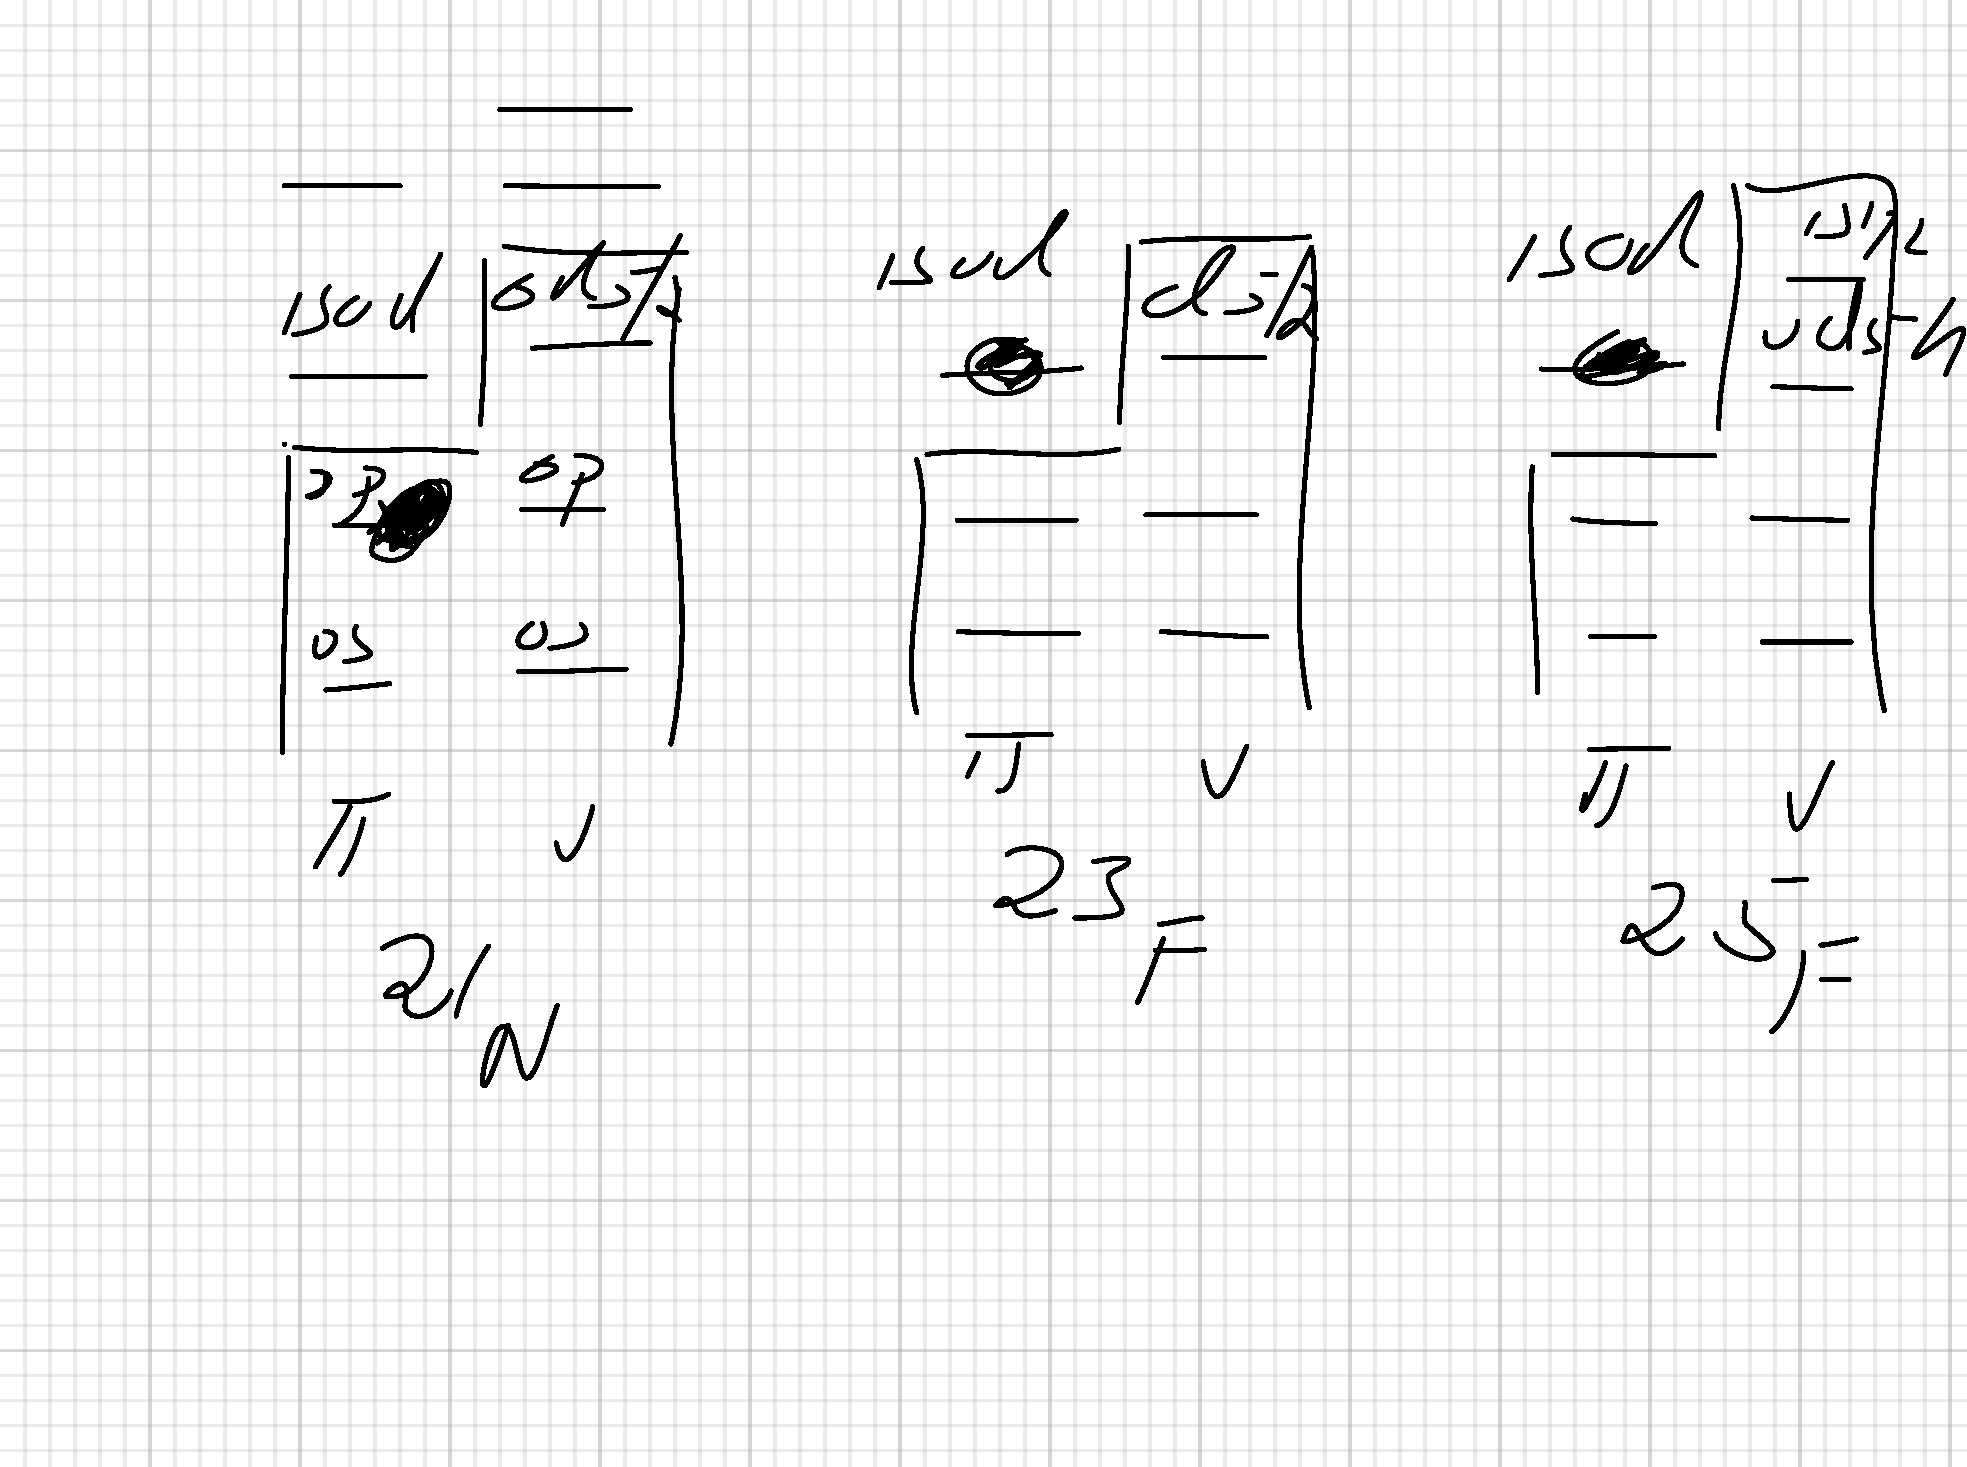
\includegraphics[width=0.6\textwidth, clip]{schematic.pdf}
	\end{center}
\caption{Possible proton states above and below the Fermi levels of  $^{23}$F, $^{21}$N, and $^{25}$F. A schematic single-particle picture has been adopted. The nucleus $^{21}$N is represented as a one-proton state removed from $^{22}$O.} 
\end{figure}


\section{Goals of the proposed experiment}
The primary goal of this experiment is to measure the spectroscopic
factors and spin-parities of states in $^{23}$F, $^{21}$N, and
$^{25}$F near the $N=14$ and $N=16$ magic numbers. By measuring proton
knockout from radioactive $^{24,26}$Ne we will be able to determine
the spectroscopic factors of the low lying states in $^{23,25}$F. This
information is crucial to the further development and predictive power
of ab initio models aiming to correctly describe the behavior of the
oxygen, and near oxygen isotopes as they approach the dripline. In
addition to the knockout from Ne, proton knockout reactions will also
be performed using a radioactive $^{22}$O beam, and a stable $^{16}$O
beam.  The aim of these reactions will be to understand the underlying
structure of the oxygen isotopes. These measurements will further
allow us to characterize the nature of the ground state of the
potentially doubly magic $^{22}$O isotope. At the same time, we will
be able to identify excited states in $^{21}$N, and make spin-parity
assignments and determine spectroscopic factors to these
states. Information on these neutron dripline nuclei, combined with
{\em ab initio} theoretical studies, will provide crucial information
to our understanding and interpetration of nuclei close to the limits
of stability. The theoretical studies will involve calculations of
spectroscopic factors from Coupled Cluster theory using $^{22}$O and
$^{24}$O as closed shell nuclei. These calculations will be
complemented with shell-model calculations using the same
Hamiltonians described in \cite{naturephysics2015,ekstrom2015}. The
effective shell-model interactions (in one or more major shells)
derived from Coupled Cluster theory are essentially parameter free
effective Hamiltonians for shell-model studies \cite{jansen2014}, including parameter free single-particle energies, as well as 
two and three-body nuclear forces.  The latter calculations
will be used to compute for example the resulting SFs between
$^{26}$Ne and $^{25}$F and $^{24}$Ne and $^{23}$F, providing thereby
an additional theoretical route to SFs and comparison with experiment. 



\begin{thebibliography}{99}

\bibitem{naturephysics2015}
{Hagen} G, {Ekstr{\"o}m} A, {Forss{\'e}n} C, {Jansen} G~R, {Nazarewicz} W,
  {Papenbrock} T, {Wendt} K~A, {Bacca} S, {Barnea} N, {Carlsson} B, {Drischler}
  C, {Hebeler} K, {Hjorth-Jensen} M, {Miorelli} M, {Orlandini} G, {Schwenk} A
  and {Simonis} J 2015 {\em Nature Physics\/} {\bf Adv. online Pub.} 1--5
  \urlprefix\url{http://www.nature.com/nphys/journal/vaop/ncurrent/pdf/nphys3529.pdf}

\bibitem{ekstrom2015}
Ekstr\"om A, Jansen G~R, Wendt K~A, Hagen G, Papenbrock T, Carlsson B~D,
  Forss\'en C, Hjorth-Jensen M, Navr\'atil P and Nazarewicz W 2015 {\em Phys.
  Rev. C\/} {\bf 91}(5) 051301
  \urlprefix\url{http://link.aps.org/doi/10.1103/PhysRevC.91.051301}

\bibitem{physicascripta2016}
G.~Hagen, G.~R.~Jansen,  M.~Hjorth-Jensen and T.~Papenbrock, Phys.~Scripta, in press (2016), arXiv1601.08203.



\bibitem{bogner2014}
Bogner S~K, Hergert H, Holt J~D, Schwenk A, Binder S, Calci A, Langhammer J and
  Roth R 2014 {\em Phys. Rev. Lett.\/} {\bf 113}(14) 142501
  \urlprefix\url{http://link.aps.org/doi/10.1103/PhysRevLett.113.142501}

\bibitem{jansen2014}
Jansen G~R, Engel J, Hagen G, Navratil P and Signoracci A 2014 {\em Phys. Rev.
  Lett.\/} {\bf 113}(14) 142502
  \urlprefix\url{http://link.aps.org/doi/10.1103/PhysRevLett.113.142502}

\bibitem{jansen2015}
{Jansen} G~R, {Signoracci} A, {Hagen} G and {Navr{\'a}til} P 2015 {\em ArXiv
  e-prints\/} (\textit{Preprint} \eprint{1511.00757})
  \urlprefix\url{http://adsabs.harvard.edu/abs/2015arXiv151100757J}
\end{thebibliography}

\end{document}






